\Chapter{A TikZ és eszközkészlete}

% Kb. 8 oldal

\Section{Ábrák szerkesztése LaTeX-ben}

\Section{A TikZ elemei}

\SubSection{Használata}

% usepackage, telepítés, útmutatók

\SubSection{Szintaxis}

% Alapvető nyelvi elemek bemutatása

\SubSection{Elérhető diagram elemek}

% Csomópontok, vonalak, feliratok, ívek, ...
% Ide kerülhetnek külön ábrák részletes magyarázatokkal (ténylegesen TikZ-s ábrák itt is).

\Section{Szerkesztőeszközök}

\SubSection{draw.io}
\begin{figure}[!h]
	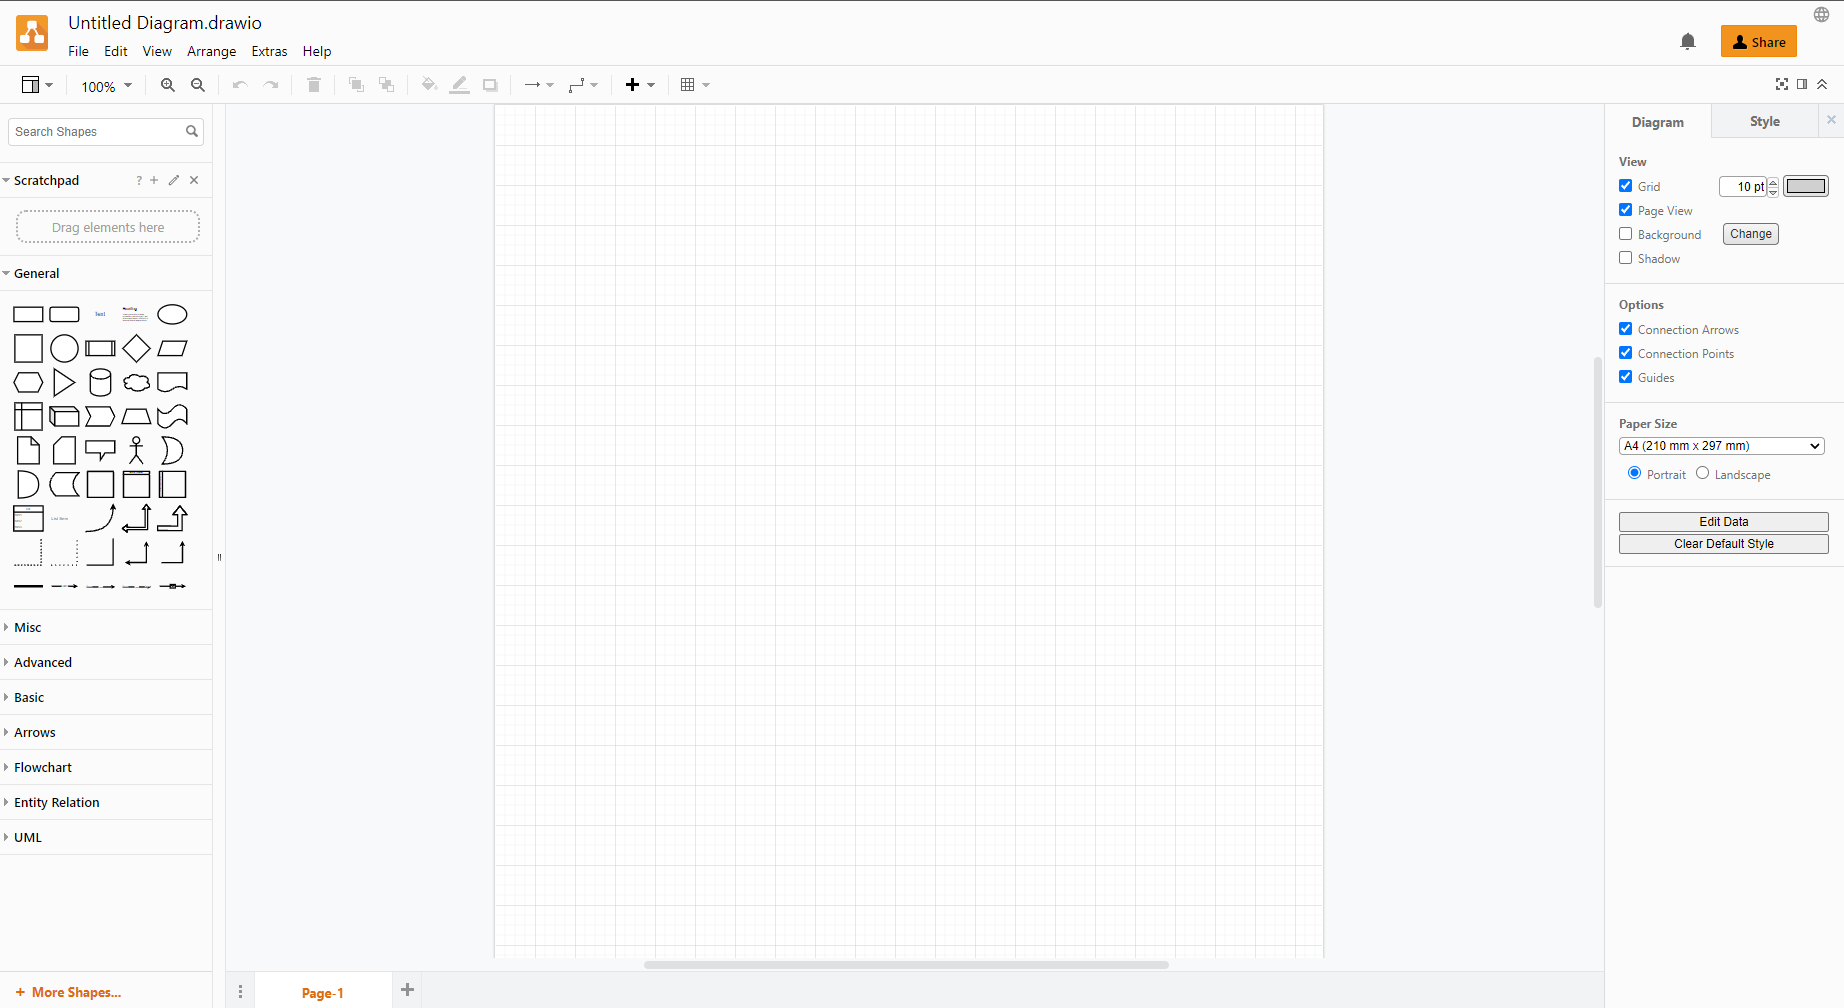
\includegraphics[width=\textwidth]{images/drawio.png}
	\caption{A draw.io kezelőfelülete \cite{drawio}}
\label{fig:drawio}
\end{figure}
A kezelőfelület fejlécében az általános menüpontok szerepelnek. Az alkalmazás közepén van maga a felület, ahol az ábrák szerkeszthetők. Ezt fogja körbe a bal oldalról az ábrákkal kapcsolatos, még jobb oldalon a diagram beállításai, és előre definiált stílusok közül lehet választani. Az alapelemek csoportosítva vannak kinézetük alapján lenyitható menüpontokként. Az ábra kiválasztása után rögtön megjelenik a felület közepén, ezt követően lehet elhelyezni. Az ábrák szerkesztésénél több lehetőség áll fenn. Rendelkezik Undo-Redo funkciókkal, az elkészített diagram menthető különböző fájlformátumokban. Az előre definiált pár stíluson felül többféleképpen is meg lehet adni saját színeket is: RGB színválasztó, hexakódok, és gyakran használt színek egyaránt. Be lehet állítani az adott ábrára kitöltőszínt, betűszínt, vízszintes és függőleges igazítást, árnyékot, bemetszést, és még sok apróságot. Bármelyik ábrára helyezhető szöveg, ennek a stílusa igazodik hozzá. Az objektumok bárhol összekapcsolhatók, de megjelennek ajánlott pontok is: 0, 25, 50, 75 és 100\%-on. A rétegek nem jelennek meg külön oldalon, az ábrák sorrendje számít, hogy melyik jelenik meg felül. A kijelölés téglalap alapú, a kijelölt elemeket lehet másolni, törölni, szerkeszteni. Az ábrák csak rácspontokhoz igazíthatók.


\SubSection{TikZiT}
\begin{figure}[!h]
	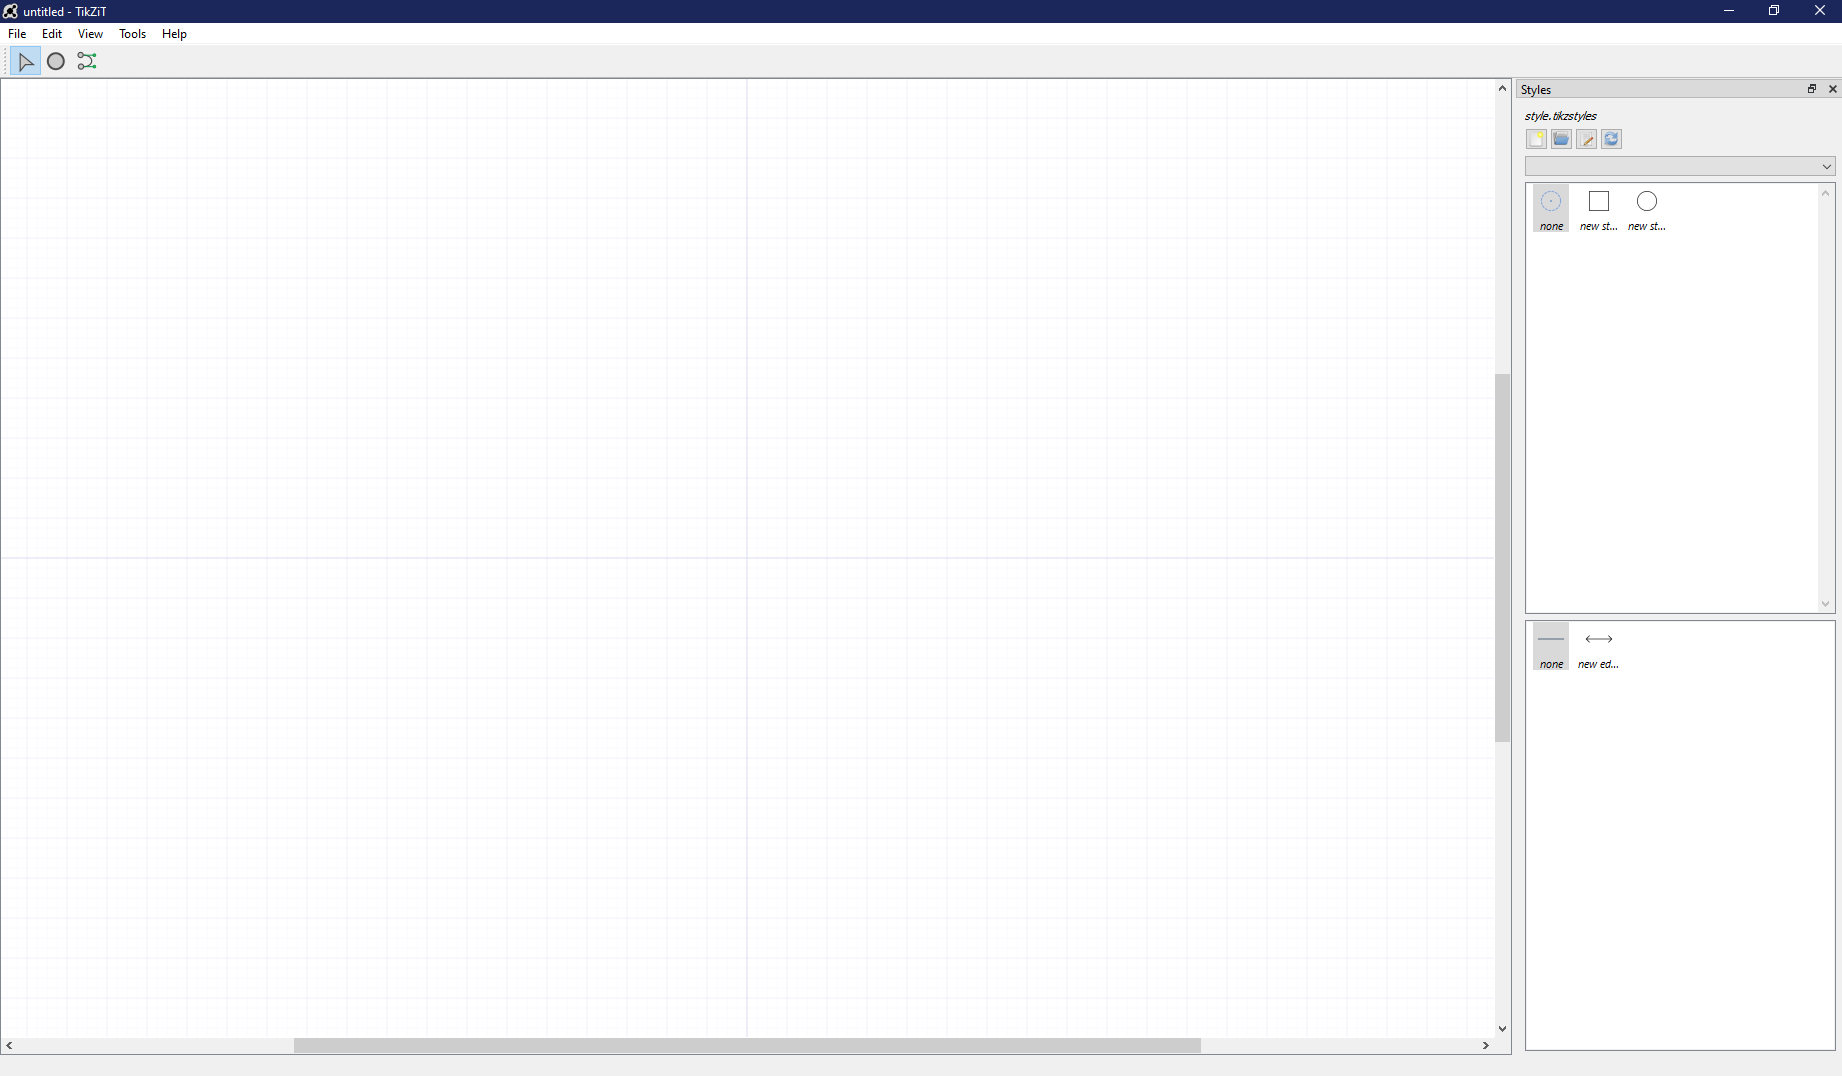
\includegraphics[width=\textwidth]{images/tikzit.png}
	\caption{A TikZiT kezelőfelülete \cite{tikzit}}
	\label{fig:tikzit}
\end{figure}
A TikZiT inkább gráfok rajzolására használható, a vezérlő elemek az alkalmazás fejlécében helyezkednek el. A grafikus alapelemek szintén itt találhatóak, számuk nem kiemelkedő: a kijelölésen kívül van egy gráf csomópont lerakásához és egy gráf éleinek berajzolásához egy gomb. Mind a csomópont, mind a gráf stílusa módosítható, fájlként menthető, és betölthető, a programon belül és kívül is szerkeszthetők. Három lehetőség van: alak, szín, kitöltés. A szín és kitöltés kiválasztása történhet előre definiált alapszínekből, de lehetőség van RGB színskálából kiválasztásra vagy hexakód megadására is. Szöveg a gráf csomópontjainak adható. A csomópontokat összekötő élek a két pont helyzetétől függenek, csak az él hajlítására van lehetőség. A csomópontok rétegződését a lerakás sorrendje határozza meg, utólag csak kijelölés után van lehetőség előre vagy hátra küldeni az adott elemet. A kijelölés téglalap alakú, a kijelölt elemek másolhatók, törölhetők, stílusuk szerkeszthető.  A program rendelkezik Undo-Redo funkciókkal, a rajzolófelületen lehetőség van nagyításra és kicsinyítésre egyaránt. A kész ábrák mentése fájlba történik, automatikus mentés nincs, ezek betölthetők későbbi szerkesztésre is. 

\SubSection{TikzEdt}
\begin{figure}[!h]
	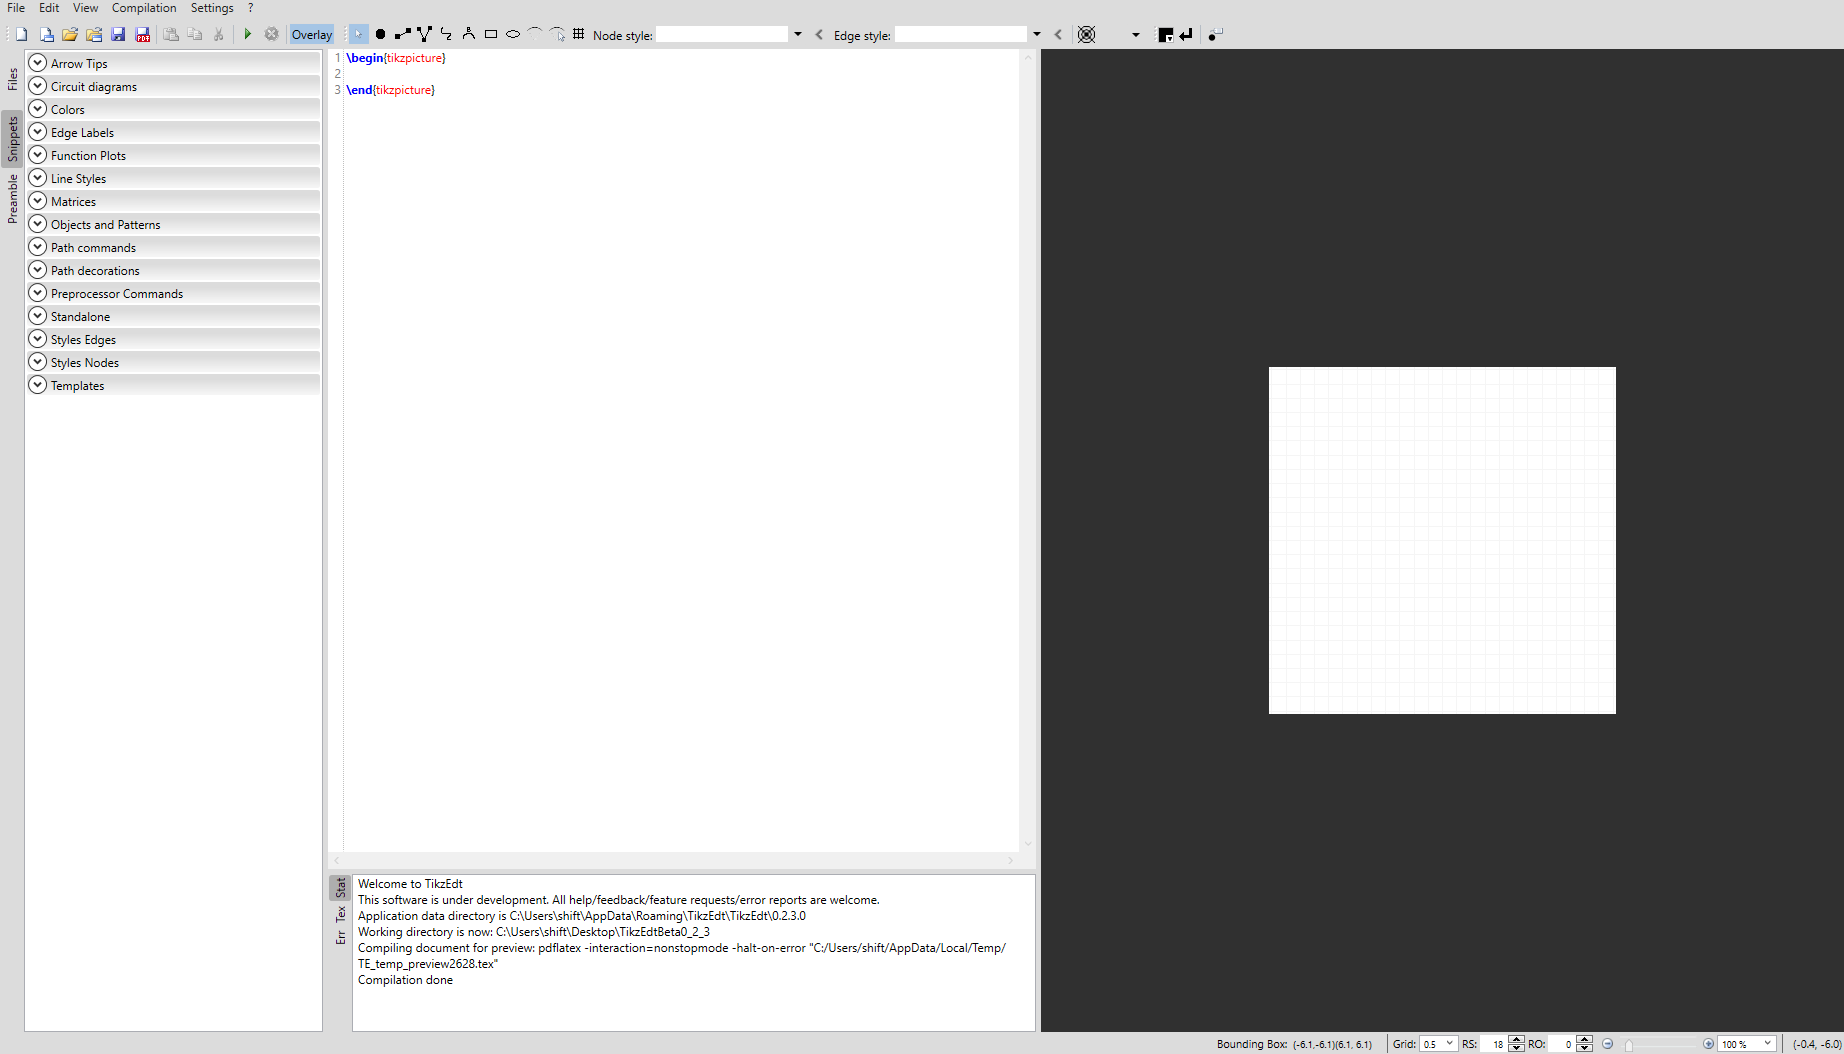
\includegraphics[width=\textwidth]{images/tikzedt.png}
	\caption{A TikzEdt kezelőfelülete \cite{tikzedt}}
\label{fig:tikzedt}
\end{figure}
A TikzEdt esetében három hasábra osztható a felület: elsőben az előre definiált LaTeX kódrészletek, másodikban a LaTeX kódszerkesztő, és végül a harmadikban a lefordított kód előnézete jelenik meg. Az alapelemek a felső sávban jelennek meg: főleg gráfokkal és egyszerűbb elemeket tartalmaz. Az elemek, gráfok, egyenletek, szövegek stílusa és színei csak kód szinten szerkeszthető, de vannak választható opciók. A rétegződés a lerakás sorrendjében van, utólag módosításra nincs lehetőség. Az elemek automatikusan rácspontokhoz igazodnak. A kijelölés téglalap alakú, a kijelölt elemek csak törölhetők.  A program rendelkezik Undo-Redo funkciókkal, a rajzolófelületen lehetőség van nagyításra és kicsinyítésre egyaránt. A kész ábrák mentése fájlba történik, automatikus mentés nincs.

\SubSection{tikzcd-editor}
\begin{figure}[!h]
	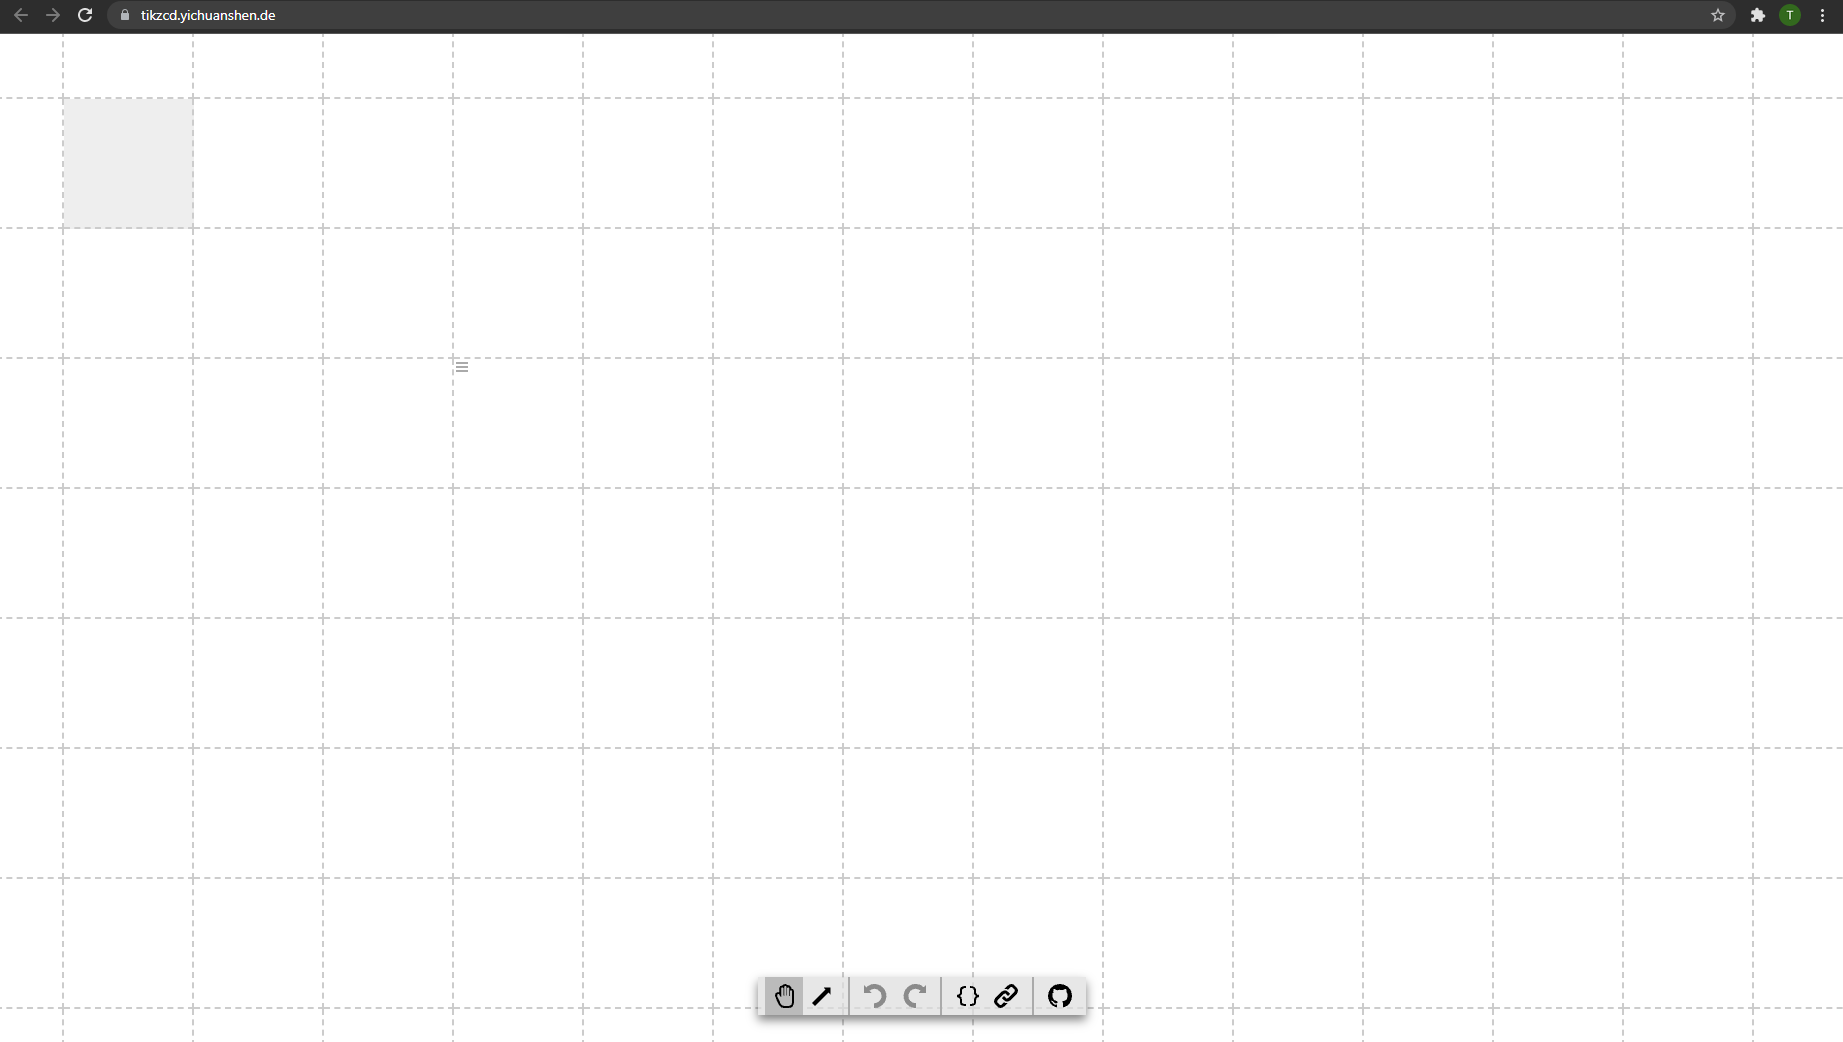
\includegraphics[width=\textwidth]{images/tikzcd.png}
	\caption{tikzcd-editor kezelőfelülete \cite{tikzcd}}
	\label{fig:tikzcd}
\end{figure}
A tikzcd-editor klasszikus felülettel nem rendelkezik, csak egy négyzet alapú rendszer fogad megnyitáskor. A rácsok közepére igazítva lehet nyilakat rajzolni, és szövegeket írni, de utólag van lehetőség a fel-le mozgatásra. A stílusok nem testreszabhatók, csak pár alap stílusból lehet választani, mint a szaggatott vagy dupla vonal, módosítható a nyíl eleje, illetve vége. Az elemek színei nem módosíthatók, csak az alap fekete érhető el. A rétegződés a lerakás sorrendjében van. Kijelölés csak egyesével működik, nincs lehetőség téglalap vagy esetleg lasszó alapú kijelölésre. A program rendelkezik Undo-Redo funkciókkal, de mentésre nincs lehetőség, csak a \LaTeX\ kód kimásolására, és az ábrához tartozó link utólagos betöltésére

% Sorban be kell mutatni, hogy milyen szerkesztőeszközök vannak.

% Képernyőképek

% Összehasonlító táblázat.
% Az összehasonlítás történhet a 3. fejezetben felsorolt szempontok szerint például.
